\documentclass[12pt]{article}
\usepackage{fancyhdr}	%More natural header control
\usepackage{graphicx}	%The graphics package. Use the command
                        %\includegraphics[width=?,height=?]{graphics_file}
			%to include graphics.  The width and height are
			%optional, and specifying one of them scales the other
			%dimension accordingly.
%\usepackage{calc}	%Use normal +-*/ notation in size specifications, etc.
\usepackage{amsmath}	%AMS math package--extra math functionality
\usepackage{amssymb}	%AMS symbol package--lots of new symbols
%\usepackage{mathptm}	%Times font w/ math
%\usepackage{mathpazo}	%Palatino font w/ math
%\usepackage{fourier}	%Utopia font w/ accompanying math
%\usepackage{multicol}	%Allows multicolumn display w/ \begin{multicols}{n}
\usepackage{amsthm}
\usepackage{textcomp}  %Access extra typesetting symbols in text mode.
\usepackage{setspace}
\usepackage{parskip}
\usepackage{amscd}
\usepackage{color}
\usepackage{ulem}
\usepackage{url}
\setlength{\voffset}{0pt}		%Top margin will be 1in + this setting
\setlength{\hoffset}{0in}		%Left margin will be 1in + this setting
\setlength{\textwidth}{6in}		%Width of the text block itself
\setlength{\textheight}{9in}		%Height of the text block
\setlength{\oddsidemargin}{0pt}	%No space for marginal notes
\setlength{\evensidemargin}{0pt}	%No space for marginal notes
\setlength{\topmargin}{0in}		%Headers will start above text
\setlength{\headheight}{0in}		%Height of header text
\setlength{\headsep}{0in}		%Separation between header and page
\setlength{\footskip}{27pt}		%Separation between footer and page
%\setlength{\parindent}{0pt}		%Amount of paragraph indentation
\setlength{\parskip}{0pt}		%Amount of skip between paragraphs
\special{papersize=8.5in,11in}		%Special to let dvips know page size
\newtheorem{theorem}{Theorem}[section]
\newtheorem{lemma}[theorem]{Lemma}
\newtheorem{example}[theorem]{Example}
\newtheorem{remark}[theorem]{Remark}
\newtheorem{definition}[theorem]{Definition}
\newcommand{\R}{{\mathbb R}}
\newcommand{\Q}{{\mathbb Q}}
\newcommand{\Z}{{\mathbb Z}}
\newcommand{\N}{{\mathbb N}}

\begin{document}
\begin{doublespace}

\begin{center}
\LARGE{Python Project}\\
\large{Econ 602, Fall 2020}\\
\large{Angelos Lagoudakis, Ezra Butcher}\\
\end{center}

A social planner maximizes%
\[
E_{t}\sum_{s=0}^{\infty }\beta ^{t}\frac{\left( c_{t+s}^{\mu }\left(
1-l_{t+s}\right) ^{1-\mu }\right) ^{1-\sigma }}{1-\sigma } 
\]%
subject to%
\[
c_{t}+k_{t+1}-\left( 1-\delta \right) k_{t}=z_{t}k_{t}^{\theta
}l_{t}^{1-\theta } 
\]%
where $z$ follows an AR(1) process:%
\[
\ln z_{t}=\rho \ln z_{t-1}+\varepsilon _{t};  \ \varepsilon _{t}\sim N\left(
0,\eta ^{2}\right) ~\mbox{i.i.d.} 
\]%
Assume the following parameter values:%
\[
\begin{tabular}{l||lll}
\hline\hline
& \multicolumn{3}{||l}{Parameter values} \\ \hline\hline
Preferences & $\mu =0.34$ & $\sigma =2$ & $\beta =0.99$ \\ 
Technology & $\theta =0.36$ & $\delta =0.025$ & $\rho =0.9;\eta =0.01$ \\ 
\hline
\end{tabular}%
\]

\begin{enumerate}
\item Discretize the productivity process into a finite state (try 5, 30)
Markov chain. You will find Python codes on the Quantecon website that can
be used for this purpose. Discretize the endogenous state $k$ into finite
grid points (try 100, 500) and use value function iteration method to obtain
value and policy functions.
\\

\item Report the value and policy functions as 3-D graphs.
\\

\item Numerically compute the stationary distribution of the capital stock
in this economy. Display the plot of this distribution.
\\

\item Report, in a table, the standard deviation of (1) GDP (2) Consumption
(3) Investment and (4) Employment. Report the autocorrelation of output and
the correlation of each of (1) consumption, (2) investment, and (4)
employment with output of this economy.
\end{enumerate}

\newpage
\begin{center}
\LARGE{Answers}
\end{center}

\begin{center}
\large{Section 1: Setup}
\end{center}

Corresponding dynamic program (Bellman): 
\[
v(z,k) = \max_{k'} \left\{u(zf(k)-k'+(1-\delta)k,1-l) + \beta E\{v(z',k')\}\right\}
\]

Labor-leisure + budget constraint: 
\[
\left(\frac{1-\mu}{\mu}\right)\left(\frac{k_{t+1}-(1-\delta)k_t}{z_t k_t^\theta}\right) = l_t^{1-\theta}\left(\frac{1-\mu}{\mu}+1-\theta-\frac{1-\theta}{l_t}\right)
\]

There's not much more to put here that would be useful, given that it's all available in the slides. \\
\\
Note that the construction of this report comes from the announcements given on Canvas and will deviate slightly from what is above.

\newpage
\begin{center}
\large{Section 2: Results}\\
\normalsize\underline{Plots of value and policy functions ($nz = 15 \mbox{ and } nk = 500$)}
\end{center}

\begin{figure}[h]
\caption{The value function was computed using Python 3.0, utilizing the method of successive approximations or as we said in class: ``value iteration." It was subject to the aforementioned budget constraint.}
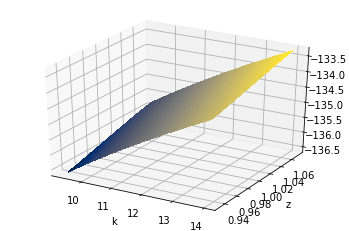
\includegraphics{3d_value_plot_nz15_nk500}
\end{figure}

\begin{figure}[h]
\caption{The associated optimal savings (capital) policy function was the following:}
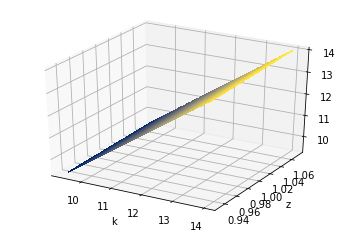
\includegraphics{3d_capital_plot_nz15_nk500}
\end{figure}

\begin{figure}[h]
\caption{Optimal GDP. We can see here that GDP is increasing in capital ($k$) for each state of the world ($z$).}
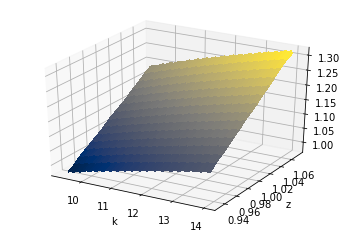
\includegraphics{3d_gdp_plot_nz15_nk500}
\end{figure}

\begin{figure}[h]
\caption{Optimal consumption. Similar to optimal GDP, consumption is increasing in capital, albeit in a much steeper way:}
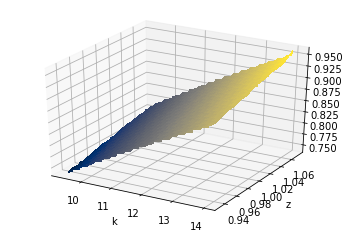
\includegraphics{3d_consumption_plot_nz15_nk500}
\end{figure}

\begin{figure}[h]
\caption{Optimal labor. Unlike GDP and consumption, labor decreases as capital increases. This makes complete sense since labor is required to install capital:}
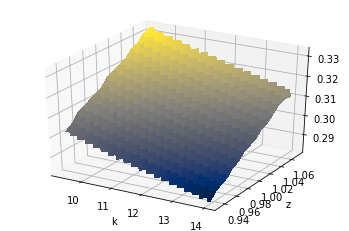
\includegraphics{3d_labor_plot_nz15_nk500}
\end{figure}

\begin{figure}[h]
\caption{Optimal investment. Like labor, this is decreasing as capital increases. Note that the rate of decrease depends more strongly on the state of the world, $z$:}
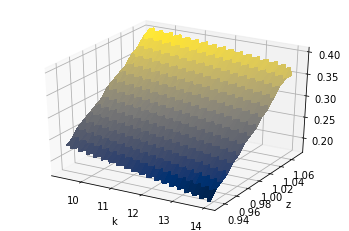
\includegraphics{3d_investment_plot_nz15_nk500}
\end{figure}

\clearpage

Similar to the model from Kydland and Prescott (1982), our model yielded observations that smoothed output, investment, consumption and labor.\\

\begin{center}
\normalsize\underline{Plots of distribution of capital stock}
\end{center}

\begin{figure}[h]
\caption{Distribution of capital stock for $nz=5 \mbox{ and } nk=100$}
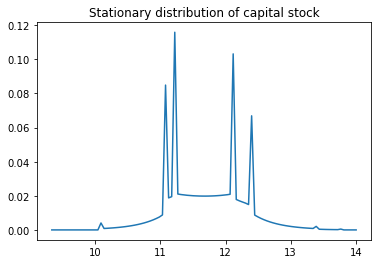
\includegraphics{capital_distribution_nz5_nk100}
\end{figure}

\begin{figure}[h]
\caption{Distribution of capital stock for $nz=5 \mbox{ and } nk=500$}
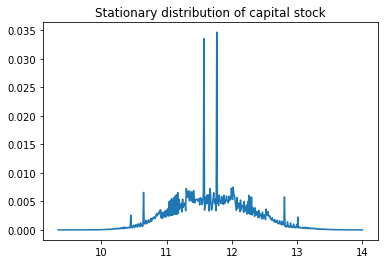
\includegraphics{capital_distribution_nz5_nk500}
\end{figure}

\begin{figure}[h]
\caption{Distribution of capital stock for $nz=30 \mbox{ and } nk=100$}
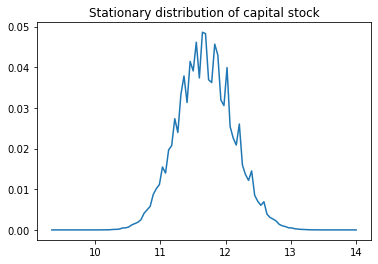
\includegraphics{capital_distribution_nz30_nk100}
\end{figure}

\begin{figure}[h]
\caption{Distribution of capital stock for $nz=30 \mbox{ and } nk=500$}
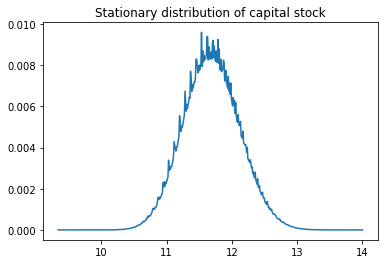
\includegraphics{capital_distribution_nz30_nk500}
\end{figure}

\clearpage

From the four plots above, we can see that $nz$ functions almost like a shape parameter, in that $nz=5$ distributions are spread out. That is, when we increase the number of states ($nz$), we can see that the distribution becomes more concentrated. For $nk$, we can see that increasing it simply makes the distribution more dense; this makes since because it's effectively just increasing the grid points. Alternatively, the law of large numbers pushes our distribution toward normality, which is to be expected because the states of the world, $z$, are lognormally distributed. \\

\begin{center}
\normalsize\underline{Result Tables}
\end{center}

%mean, std, volatility, autocorrlations for labor, cons, inv, gdp, capital
\begin{center}
\begin{tabular}{ |p{2.5cm}|p{2.25cm}|p{2.25cm}|p{2.25cm}|p{2.25cm}|p{2.25cm}|  }
 \hline
 \multicolumn{6}{|c|}{Descriptive Statistics} \\
 \hline
 Variables & Labor & Consumption & Investment & GDP & Capital\\
 \hline
 Mean & 0.3071 & 0.0210 & 0.2922 & 1.1389 & 11.687 \\
 St. Dev. & 0.0047 & 0.021 & 0.0292 & 0.0457 & 0.439 \\
 Volatility (\%) & 1.525 & 2.478 & 9.98 & 4.009 & 3.756 \\
 Autocorr. & 0.8552 & 0.9802 & 0.8766 & 0.9247 & 0.9981 \\
 \hline
\end{tabular}
\end{center}

\bigskip
%correlations
\begin{center}
\begin{tabular}{ |p{2.25cm}|p{2.25cm}|p{2.25cm}|p{2.25cm}|p{2.25cm}|p{2.25cm}|  }
 \hline
 \multicolumn{4}{|c|}{Correlations} \\
 \hline
 &Labor&Consumption&Investment\\
 \hline
 GDP&0.8366&0.8739&0.9368\\
 \hline
\end{tabular}
\end{center}

\bigskip
\begin{center}
\normalsize\underline{Volatilities}
\end{center}

\begin{itemize}
\item Consumption's volatility is lower than the volatility of output (GDP). We can expect this since the consumption patterns don't change as rapidly as the output of an economy going through a shock. Mathematically, we can see this in the budget constraint because the state of the world, $z$, affects consumption indirectly since we can write consumption as $c = zk^\theta l^{1-\theta} -k' + (1-\delta)k$. That is, consumption is buoyed by the investment term.
\item Investment has the highest volatility of all the variables. According to Auerbach (2020), the nature of the investment process is what leads volatility to high levels. Investment decision-making requires longer times and often is consequential in an order of magnitude larger than consumption, e.g. a cheeseburger vs. a home. So, during times of recession, investment is the first to go, while consumption lags (ceteris paribus).
\item Labor has the lowest volatility of all the variables. Intuitively, we can think of this as labor being ``sticky"---that people continue to work similar amounts regardless of output and the general state of the world. Since labor is restricted by physical limits (only 24 hours in a day), it makes sense that the volatility must be lower because it's inherently bounded.
\end{itemize}

\begin{center}
\normalsize\underline{Persistence}
\end{center}

\begin{itemize}
\item Output persistence (autocorrelation of GDP) is $0.9247$, and persistence for $z$ ($\rho$) is $0.9$. Practically, we know that $z$ follows an $AR(1)$ process; hence, we can expect output to be correlated in the same manner.
\item Labor in our model is not more persistent than $z$; however, consumption is more persistent than $z$. This relates back to the notion of ``sticky" consumption patterns. For labor, it would make sense to have the highest persistence, given lower volatility and the notions mentioned above, but that wasn't reflected in our output.
\item Since we have ``creative freedom," we decided to think about the relationship between labor and capital persistence. Specifically, when capital persistence is high (similar across periods), it makes sense for labor persistence to be low since they are in a sense substitutable components of output.
\end{itemize}

\begin{center}
\normalsize\underline{Correlations}
\end{center}

\begin{itemize}
\item As expected, investment (capital savings) has a high correlation with output. This makes sense because firms investing has a direct effect on output, given that we do not have a productivity or technology parameter affecting output.
\item Consumption correlates highly with output. Historically, the expenditure approach has been a popular method for measuring GDP. This makes sense because consumer spending is normally the largest component of GDP, particularly in the United States. 
\item Labor correlates the lowest with GDP of the three variables measured. Measuring the effect of labor on output is more difficult than either consumption or investment due to labor often taking place outside the market economy, e.g. domestic engineering. Furthermore, the inclusion of instrumental variables could increase this correlation.
\end{itemize}

\newpage
\begin{center}
\LARGE{Section 3: Conclusions}
\end{center}

\begin{center}
\normalsize\underline{What We Did}
\end{center}

We utilized a dynamic programming model to analyze a hypothetical economy and explain the relationships between key economic variables and GDP. In addition, we explored the persistence and volatility (\% rate of change) of each key component of the economy. We concluded that investment has the largest effect on output, and capital is the most persistent economic variable in this model. Additionally, investment, being the most consequential, was also the most volatile. Conversely, labor demonstrated the least volatility while also having the lowest correlation with output. The performance of this model shows room for improvement with the inclusion of parameters accounting for technology and productivity changes over time. Dynamic models, such as the one in this project, are capable of predicting the consequences of specific shocks to the economy and informing policymakers of the ramifications of intervention.

\begin{center}
\normalsize\underline{What We Learned}
\end{center}

This was overall an interesting project which helped us develop coding skills, good team work habits, and a creative spirit. You stated that ``Macro is not for poets." We disagree with this statement, as we many times felt like poets during the last week---albeit not good ones. On a more serious note, both of us have backgrounds in statistical computing---Angelos in academia and Ezra in the private sector---but this project demonstrated the usefulness of dynamic programs in solving complex models. Moreover, connecting the concepts from class with a practical problem helped to solidify what we learned. 

\newpage
\begin{center}
\LARGE{References}
\end{center}

\begin{itemize}
\item Auerbach, A. J. (n.d.). Investment. Retrieved December 05, 2020, from \url{https://www.econlib.org/library/Enc1/Investment.html}
\item Kydland, F. E., \& Prescott, E. C. (1982). Time to build and aggregate fluctuations. Econometrica: Journal of the Econometric Society, 1345-1370.
\end{itemize}




\end{doublespace}
\end{document}